\section{Viewing and Cleaning the Data}
\label{sec:clean}
\fix{George's section: The two views of GPU life: by SN and by
  location, its use in cleaning data, etc.}

As we need to recover durations from this data, correct processing
involves time adjustments for switching between daylight saving time
and standard time. We perform this by setting a reference time zone
(Eastern time) and converting all date-times from strings into
date-time variables \fix{(is there a name for this?)} with the R
\pkg{lubridate} package \cite{lubridate}, which enables appropriate
date arithmetic.

\fix{Other processing:} enable missing values, and create some new
variables. The event is “life” when both insert and remove are
present, “life0” when insert = remove, otherwise it is whatever string
is in insert, which is “DBE” or “Off The BUS”. Also separate location
into its components and fill in (repeat) serial numbers and locations
for all records.

Reduce to only “life” records and mark them with ending DBE, OTB,
“out”, or none events. The result is just insert and remove with event
marks to indicate DBE or OTB or “out” (last seen). bad indicates that
a DBE or OTB occurred yet the GPU was not taken out. For a first cut,
keep the bad ones in. Also keep duration to later aggregate into full
life times.

Next, aggregate into one record per serial number with total life time
and first insert time. For proper censoring treatment: Indicate if
event occurred or still in service: out = fail, dbe = fail, otb =
fail, NA = right censored (still in service). Add some other
variables, such as GPU in single location or moved one or more times,
mark new\_batch group, etc. to use in modeling later.

To get some intuition for the GPU lifetimes on Titan, we give two views of
a hundred GPUs (Figure~\ref{fig:gpuview}) and a hundred locations
(Figure~\ref{fig:locview}). The GPU view is ``by serial number'' that
shows when each GPU was installed and removed at various locations as
well as its DBE and OTB events. The second view by location, shows
when different GPUs were installed and removed at a location, and
their OTB and DBE events.
\begin{figure}[ht]
  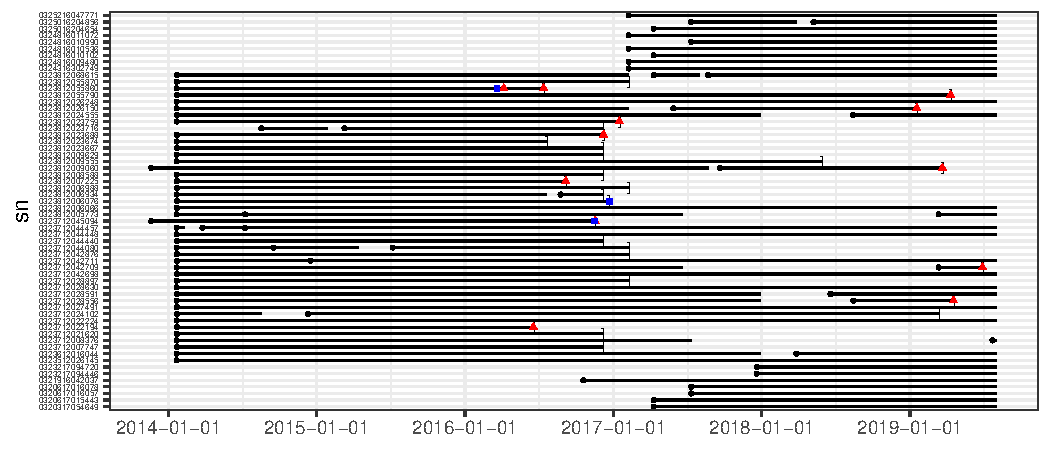
\includegraphics[width=6in]{figs/sample_sn.pdf}
  \caption{GPU serial number view of life and failures. Legend: black
    dots are installs, black lines are lifetimes at installed
    location, blue squares are OTB events, red triangles are DBE
    events, and black ] are ``last seen'' events.}
  \label{fig:gpuview}
\end{figure}
\begin{figure}[ht]
  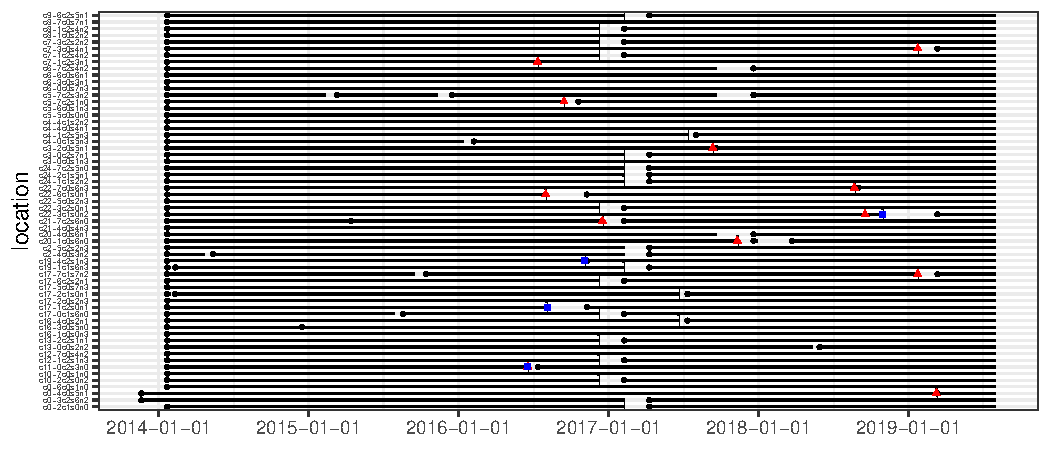
\includegraphics[width=6in]{figs/sample_loc.pdf}
  \caption{GPU location view of life and failures.  Legend: black
    dots are installs, black lines are lifetimes at installed
    location, blue squares are OTB events, red triangles are DBE
    events, and black ] are ``last seen'' events.}
  \label{fig:locview}
\end{figure}
The serial number view clearly shows the two batches and the more
frequent OTB and DBE events in the old batch. It is also clear from
this view that most new GPUs stay at the initial install location
whereas the old GPUs were occasionally reinstalled at new locations.
The location view shows that each location was operational almost all
the time with small gaps when GPUs were changed out.

\fix{Were the GPUs swapped out as a blade or were individual GPUs
  swapped on a blade?}
